\section{Декартово ГП. Семантическое ГП.}
Идея декартово генетического программирования: структуры программы дана, нужно лишь заполнить ее операторами и ссылками на переменные.
Общий вид:
\begin{figure}[h]
\centering
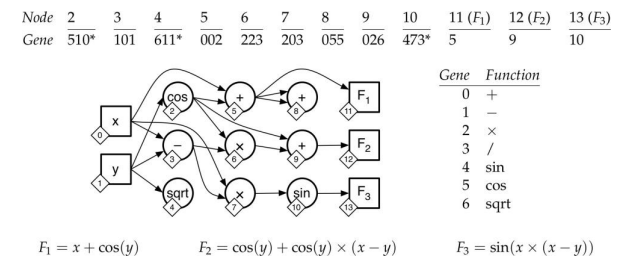
\includegraphics[width=0.8\linewidth]{images/decart.png}
\caption{Пример}
\label{fig:mpr}
\end{figure}
Ограничение в изначальном наборе операторов. 
Семантическое генетическое программирование. Основная идея состоит в том что мы хотим изменять не гены которые могут изменять сильно фенотип а непосредственно сам фенотип. 
Для этого используются следующие подходы:
\begin{itemize}
	\item Обертки (Wrappers). Стандартные операторы, проверяем семантику, при необходимости повторяем. При необходимости: либо тождественно родителю, либо сильно отличается
	\item Операторы, которые в курсе семантики. Пример: обмен только семантически схожих (но не идентичных) поддеревьев
	\item Инициализация, которая в курсе (Semantic-aware initialization). Порождает семантически разнообразные начальные популяции Пример: если поведение особи похоже на уже имеющееся, пересоздаем
	\item «Геометрические» операторы. 
	\begin{itemize}
		\item Мутация: семантика внутри окрестности семантики родителя
		\item Скрещивание: семантика на отрезке между семантикой родителей
		\item Определения окрестности и отрезка зависит от используемой метрики
		\item Преимущество: Оптимизация делается просто, так как функция приспособленности упрощается или даже становится унимодальной
		\item Недостаток: высокий рост размера программы
	\end{itemize}
\end{itemize}
